\documentclass[a4paper, 12pt]{article}

\usepackage[T2A]{fontenc}
\usepackage[english, russian]{babel}
\usepackage[top=2cm,bottom=3cm,left=1.5cm,right=1.5cm]{geometry}

% Пакет для расширения возможностей
% работы с формулами
\usepackage{amsmath}

% Расширение набора
% математических символов
\usepackage{amsfonts}
\usepackage{amssymb}

% Подключим пакет, отвечающий
% за изображения
\usepackage{graphicx}

\usepackage{indentfirst}

\graphicspath{ { ./images/ } }

% Попробуем подвигать текст вручную
% (тут мы будем двигать на титульном листе,
% но аналогичные операции будут работать
% везде в теле документа)
\begin{document}

\title{Отчёт о выполнении лабораторной работы 1.1.4 \\
Изучение статистических закономерностей на примере измерения фона космического излучения}
\author{Новиков Александр, Б03-603}
\maketitle

\section{Аннотация}

В работе исследуются статистические закономерности на примере измерения
естественного радиационного фона. Проверяется согласованность полученных данных
с теоретическими распределениями Пуассона и Гаусса.

В работе используется счётчик Гейгера-Мюллера и компьютер для связи со
счётчиком.

\section{Теоретические сведения}
\begin{figure}[h]
	\label{fig:geiger}
	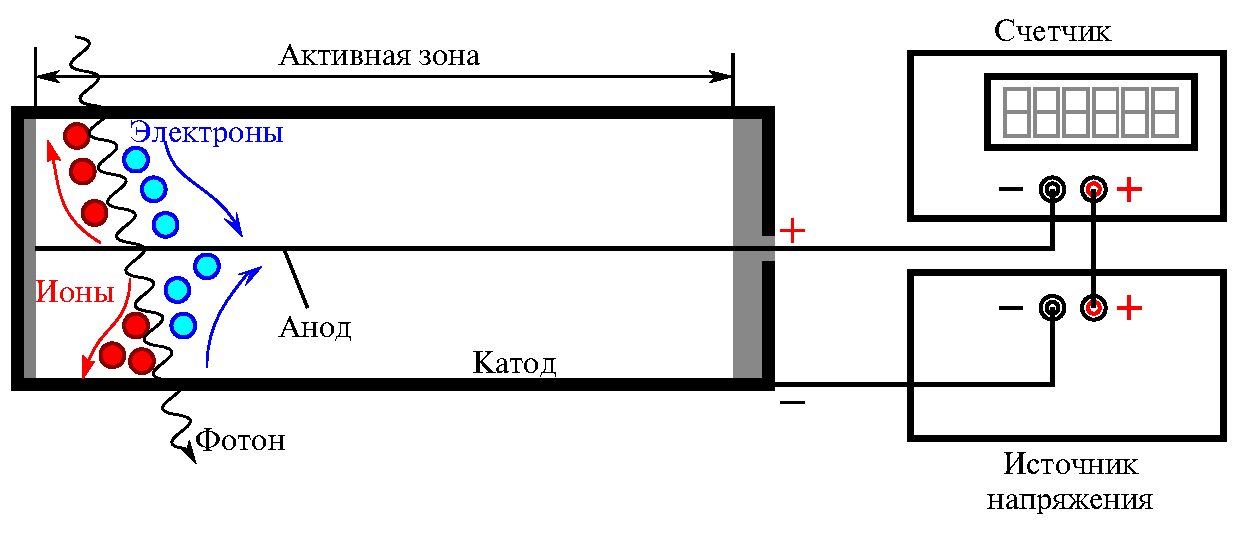
\includegraphics[width=\textwidth]{images/geiger.pdf}
	\caption{Принципиальная схема счётчика Гейгера-Мюллера.}
\end{figure}
Для обнаружения фоновых частиц используется счётчик Гейгера-Мюллера. Он
представляет собой наполненный газом сосуд с двумя электродами. В работе
используется счётчик СТС-6, который представляет собой металлический цилиндр
(катод) с нитью, натянутой вдоль оси цилиндра (анод). На электроды подаётся
напряжение порядка 400 В. Пролетающие частицы ионизируют газ в цилиндре
и выбивают электроны из его стенок. В результате ток, проходящий через счётчик,
значительно усиливается, что фиксируется компьютером, подключенным к счётчику.
Схема счётчика представлена на рисунке \ref{fig:geiger}.

Пролёты частиц через счётчик однородны во времени, и частицы почти не влияют
друг на друга. Такой процесс называется пуассоновским. В теории вероятностей
доказывается, что такой процесс удовлетворяет распределению Пуассона.
Вероятность, что в какой-то момент времени будет обнаружено $n$ частиц, 
оперделяется формулой:
\begin{equation}
	\label{puasson}
	w_n=\frac{{\overline{n}}^n}{n!}e^{-\overline{n}}
\end{equation}

Ключевое свойство этого распределения — равенство дисперсии среднему значению:
\begin{equation}
    \sigma_n^2 = \overline{n} \implies \sigma_n = \sqrt{\overline{n}}
\end{equation}

При $n\rightarrow \infty$ распределение Пуассона переходит в распределение
Гаусса, $w_x$ --- функция плотности распределения вероятности:
\begin{equation}
	\label{gauss}
	w_x=\frac{1}{\sqrt{2\pi}\sigma_n}
	e^{-{\frac{(x-\overline{n})^2}{2\sigma_n^2}}}
\end{equation}

\section{Методика измерений}

%\subsection{Приборы}
%\begin{itemize}
%    \item Счётчик Гейгера-Мюллера.
%%    \item Блок питания и повышающий трансформатор.
%%    \item Плата аналого-цифрового преобразователя (АЦП).
%    \item ПК с интерфейсом для связи со счётчиком.
%\end{itemize}

%\begin{figure}[h]
%    \centering
%    
\includegraphics[width=\textwidth]{images/installation}
%    \caption{Установка.}
%    \label{fig:installation}
%\end{figure}

%\subsection{Процедура измерений}
Мы непрерывно считаем импульсы со счётчика, сигнал оцифровывается и летит на ПК.
Программа фиксирует количество импульсов каждую секунду ($\tau_0 = 1$~с).
При обработке этот сырой массив склеивается в более крупные блоки 
($\tau = 10, ~20, ~40, ~80$~с),
после чего для каждого интервала считается статистика
и строятся гистограммы частот $w_n = N_n / N$.

\section{Результаты измерений}

На рисунке \ref{fig:hist} представлены гистограммы частот для всех интервалов группировки,
поверх которых наложены идеальные теоретические кривые Пуассона и Гаусса
для базового распределения ($\tau = 20$ с).

\begin{figure}[h]
    \centering
	%\makebox[\textwidth][c]{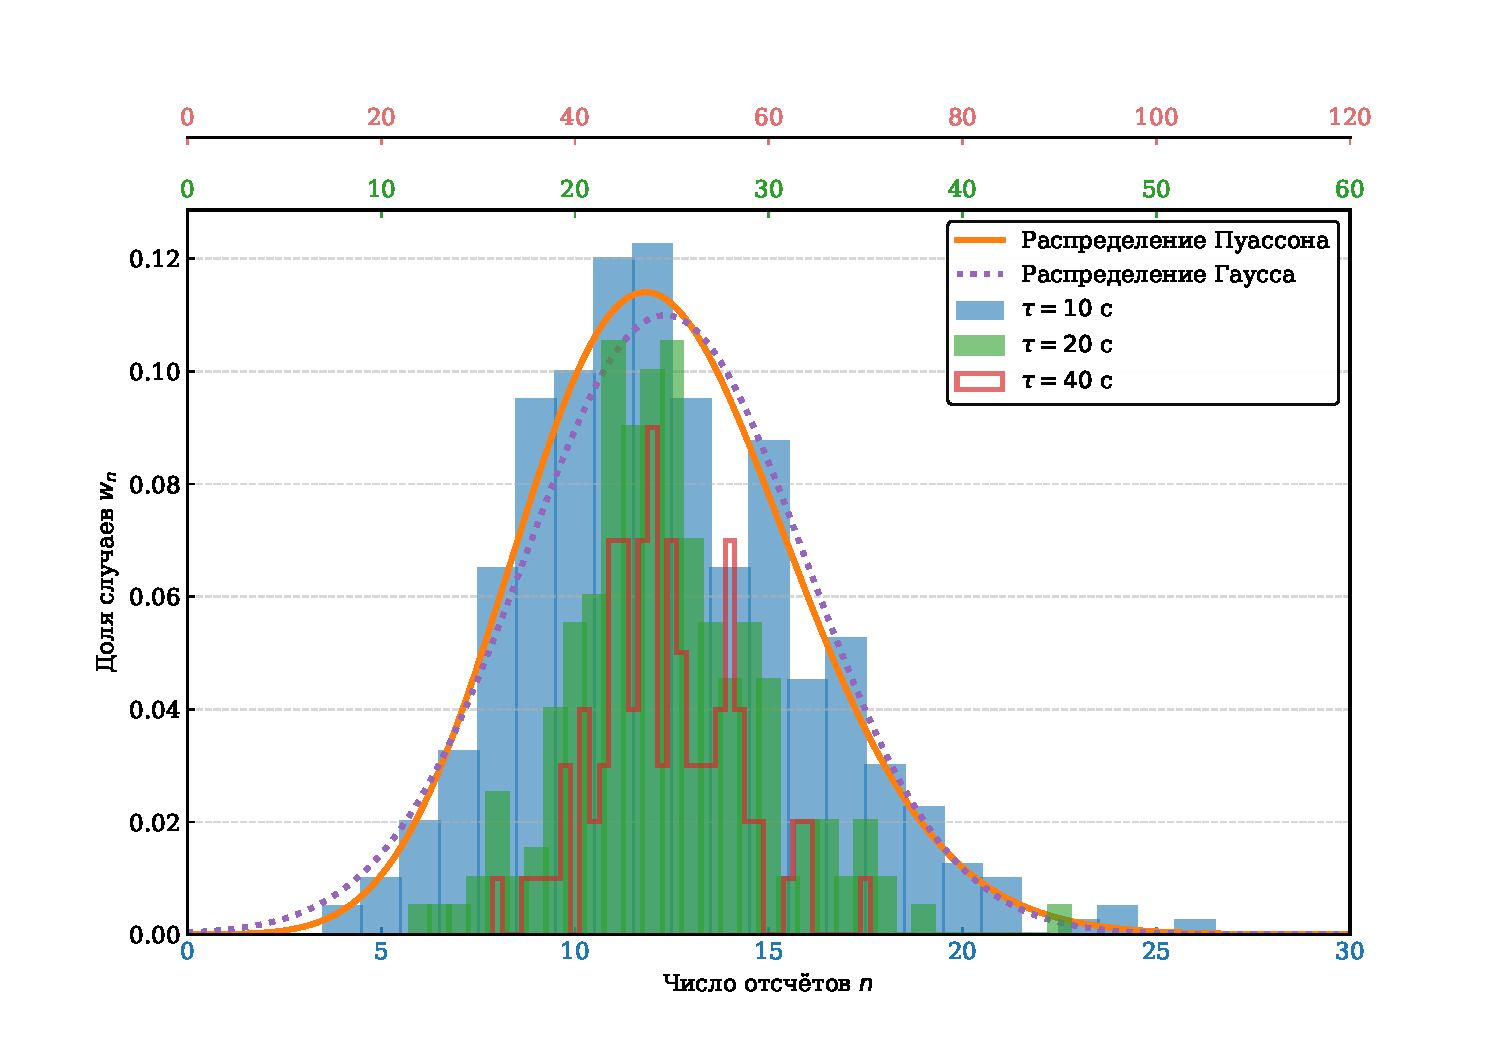
\includegraphics[width=1.4\textwidth]{images/gauss}}
	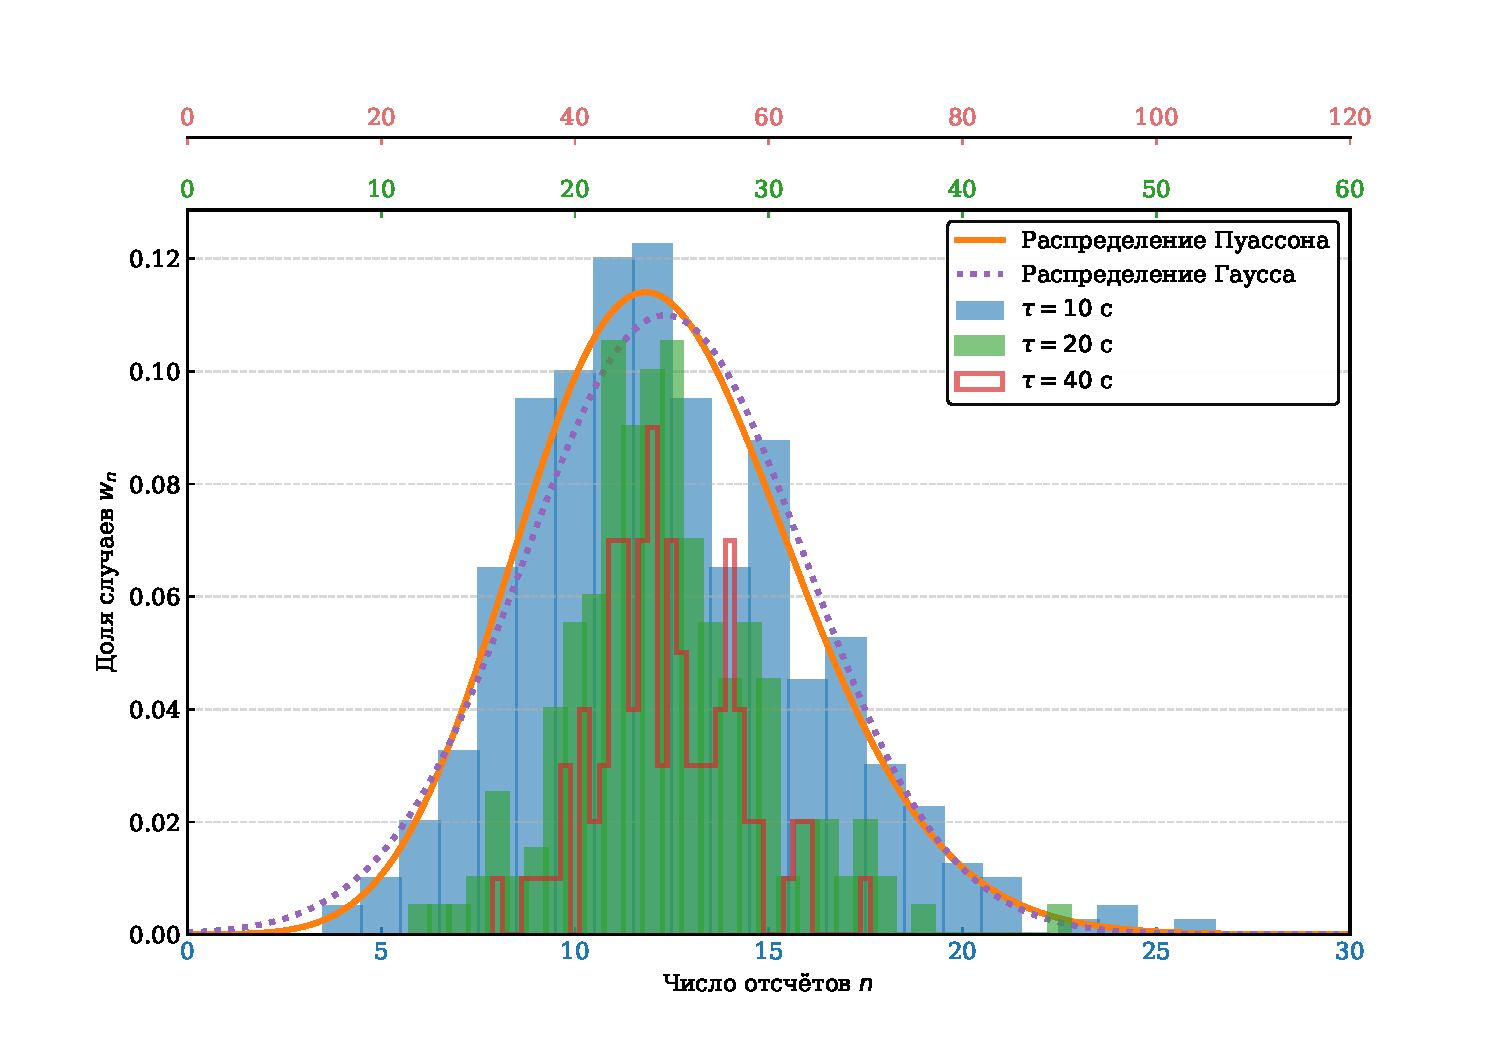
\includegraphics[width=\textwidth]{images/gauss}
    \caption{Гистограммы распределения количества частиц для $\tau = 10, 20, 40, 80$ с и теоретические распределения для $\tau = 10$ с.}
    \label{fig:hist}
\end{figure}

Проверяем «правило сигм» на примере разбиения $\tau = 20$ с.
Из общего числа $N = 200$ интервалов:\nopagebreak
\begin{enumerate}
	\item В интервал $\pm 1 \sigma_n$ попало 148 отсчётов (74\%). Теоретическое ожидание: 68\%.
	\item В интервал $\pm 2 \sigma_n$ попало 189 отсчётов (94{,}5\%). Теоретическое ожидание: 95\%.
	\item В интервал $\pm 3 \sigma_n$ попало 199 отсчётов (99{,}5\%). Теоретическое ожидание: 99{,}7\%.
\end{enumerate}

Сгруппируем данные и для каждой группы посчитаем
среднее число регистрируемых частиц $\overline{n}$,
среднеквадратичное (стандартное) отклонение $\sigma_n$,
погрешность среднего значения $\sigma_{\overline{n}}$.
Полученные данные занесём в таблицу \ref{tab:groups}.

\begin{table}[h]
    \caption{Значения $\overline{n}$, $\sqrt{\overline{n}}$, $\sigma_n$, $\sigma_{\overline{n}}$ для каждой из групп.}
	\begin{tabular}{|c|r|r|r|r|}
	\hline
	\textbf{$\tau$, с} & \multicolumn{1}{c|}{\textbf{$\overline{n}$}} & \multicolumn{1}{c|}{\textbf{$\sqrt{\overline{n}}$}} & \multicolumn{1}{c|}{\textbf{$\sigma_n$}} & \multicolumn{1}{c|}{\textbf{$\sigma_{\overline{n}}$}} \\ \hline
	1                  & 1{,}232                                      & 1{,}110                                             & 1{,}124                                  & 0{,}018                                               \\ \hline
	10                 & 12{,}322                                     & 3{,}510                                             & 3{,}629                                  & 0{,}181                                               \\ \hline
	20                 & 24{,}645                                     & 4{,}964                                             & 4{,}892                                  & 0{,}346                                               \\ \hline
	40                 & 49{,}290                                     & 7{,}021                                             & 6{,}939                                  & 0{,}694                                               \\ \hline
	80                 & 98{,}580                                     & 9{,}929                                             & 10{,}006                                 & 1{,}415                                               \\ \hline
	\end{tabular}
    \centering
    \label{tab:groups}
\end{table}

Средняя интенсивность регистрируемых частиц:
$$j = 1{,}232 \pm 0{,}018 ~\frac{\text{частиц}}{\text{с}}$$

На рисунке \ref{fig:screen} представлены четыре основных графика, реализуемых в программе:
зависимость числа отсчётов от времени, гистограмма результатов,
а также зависимости накопленного среднего
и погрешности (в логарифмическом масштабе) от номера измерения.

\begin{figure}[h]
    \centering
	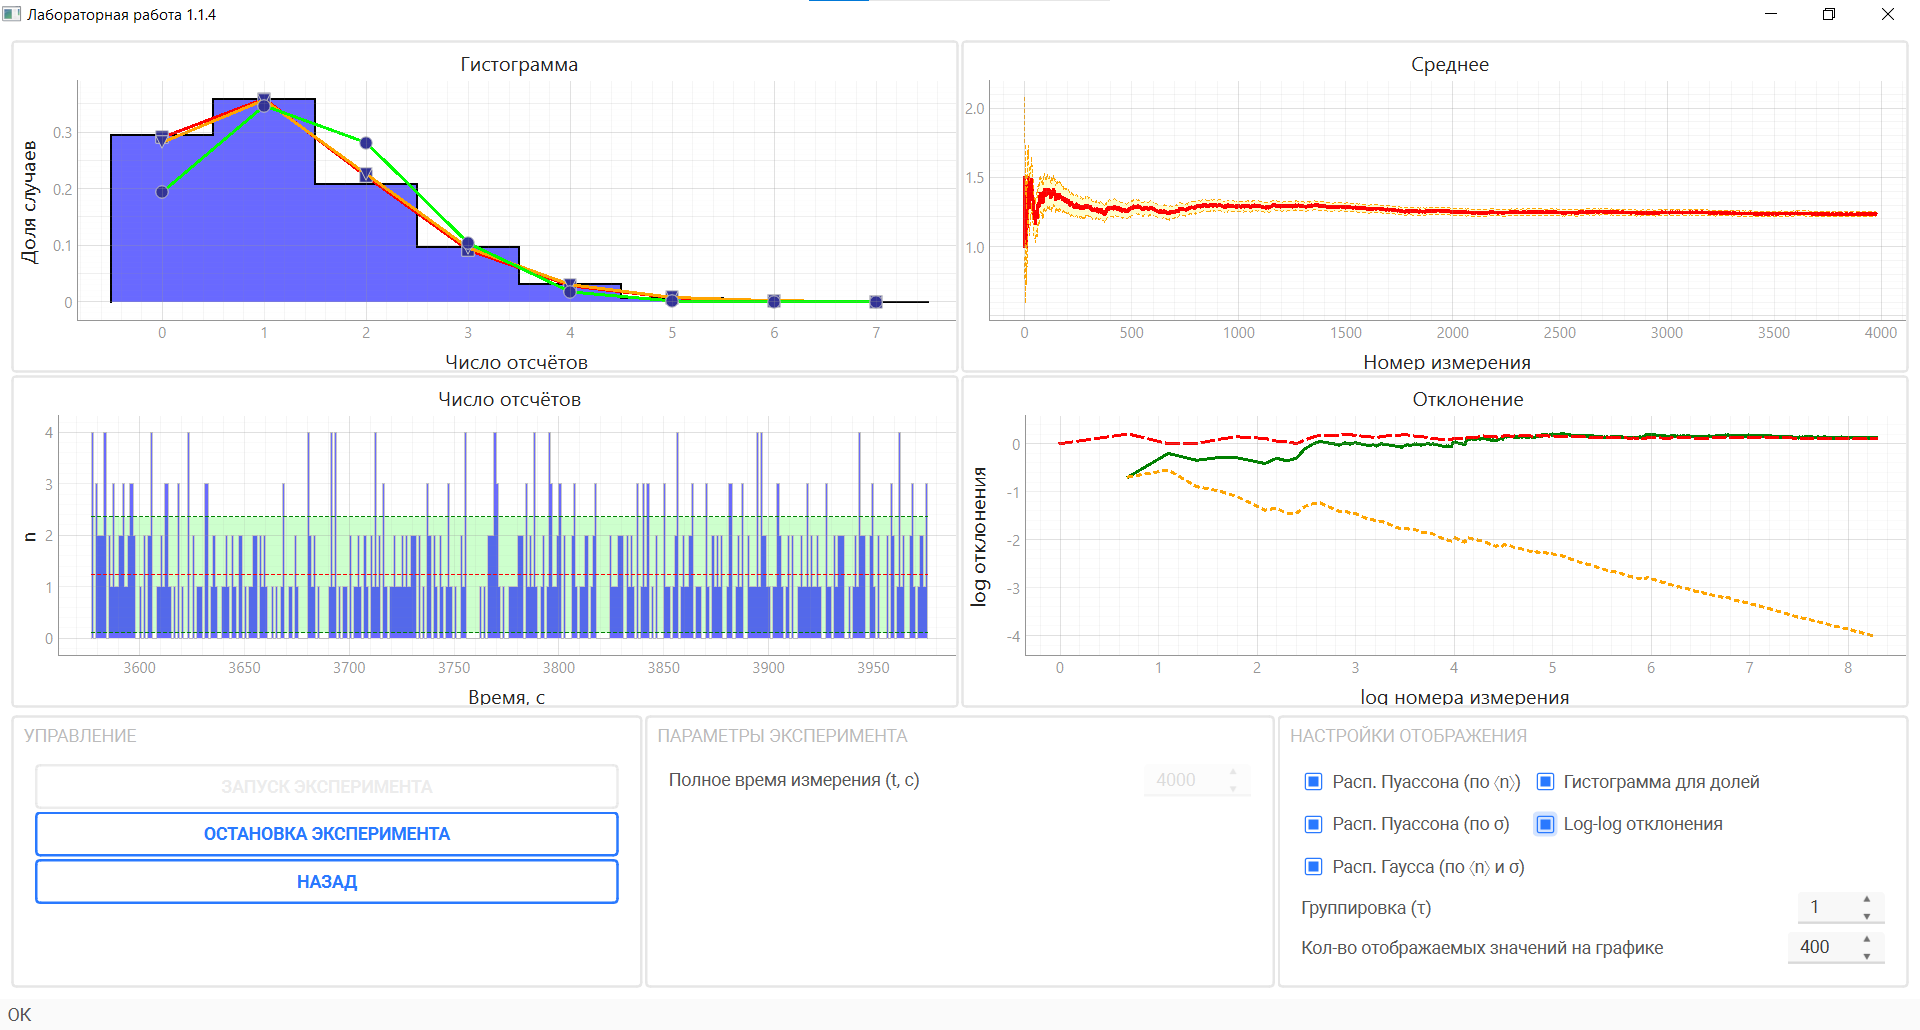
\includegraphics[width=\textwidth]{images/screenshot}
    \caption{Интерфейс программы со статистическими характеристиками случайного процесса.}
    \label{fig:screen}
\end{figure}

\section{Обсуждение результатов}

В процессе измерения можно наблюдать, что с увеличением времени
и, соответственно, числа измерений:
\begin{enumerate}
	\item Количество частиц в секунду флуктуирует,
	\item Среднее значение количества частиц в секунду
	приближается к постоянному значению, 
	\item Гистограмма распределения количества частиц в интервал 
	времени приближается к пуассоновскому распределению, 
	\item Стандартное отклонение тоже стремится к постоянному значению.
\end{enumerate}

Заметим, что для всех групп
$\sigma_{\overline{n}} \approx \sqrt{\overline{n}}$
с точностью до $0{,}1$.
Основное свойство распределения Пуассона выполнено.
Значит, мы наблюдаем действительно пуассоновский процесс.

Правило «трёх сигм» для $\tau=20$ с выполняется весьма точно
— наши проценты (74\%, 94{,}5\%, 99{,}5\%) очень близки к идеальным гауссовским.

Относительная погрешность $\varepsilon \approx 1.4\%$ не зависит от группировки данных.

На правом нижнем графике (рис. \ref{fig:screen})
представлена зависимость $\log(\sigma_{\overline{n}})$ от $\log(N)$.
Она представляет собой прямую линию с коэффициентом $-0{,}5$,
что подтверждает зависимость %\linebreak[4]
$$\sigma_{\overline{n}} = \frac{\sigma_n}{\sqrt{N}}$$

Это экспериментально подтверждает фундаментальный закон:
для повышения точности измерений в 10 раз
необходимо увеличить время сбора статистики в 100 раз.

\section{Заключение}

В работе измерено среднее число частиц, прошедшее через счётчик Гейгера-Мюллера
и проверено выполнение статистических закономерностей, таких как законы
распределения Пуассона и Гаусса, которые наиболее точно описывают распределение
среднего числа частиц, возникшее при обработке данных измерений.

\end{document}